\documentclass[a4paper,14pt]{article}
\usepackage[14pt]{extsizes}




\usepackage{cmap}					% поиск в PDF
\usepackage{mathtext} 				% русские буквы в формулах
\usepackage[T2A]{fontenc}			% кодировка
\usepackage[utf8]{inputenc}			% кодировка исходного текста
\usepackage[english,russian]{babel}	% локализация и переносы
\usepackage{ulem}                   % зачеркнутый текст
\usepackage{amssymb}			% пакет математики
\usepackage{float}
\usepackage{amsmath}
\usepackage{graphicx}
\DeclareGraphicsExtensions{.png}

%%% Страница
%\usepackage{extsizes} % Возможность сделать 14-й шрифт
\usepackage[left=1cm,right=1cm,top=1cm,bottom=1cm]{geometry} % Простой способ задавать поля
\pagestyle{empty}

\begin{document}


\begin{center}
ФЕДЕРАЛЬНОЕ ГОСУДАРСТВЕННОЕ ОБРАЗОВАТЕЛЬНОЕ БЮДЖЕТНОЕ УЧРЕЖДЕНИЕ ВЫСШЕГО ОБРАЗОВАНИЯ

    \textbf{«ФИНАНСОВЫЙ УНИВЕРСИТЕТ ПРИ ПРАВИТЕЛЬСТВЕ РОССИЙСКОЙ ФЕДЕРАЦИИ»}

Факультет информационных технологий и анализа больших данных

Департамент анализа данных и машинного обучения

\textit{
	\textbf{Дисциплина: «Теория вероятностей и математическая статистика»}}

\textit{Направление подготовки: 01.03.02 «Прикладная математика и информатика»}

\textit{Профиль: «Анализ данных и принятие решений в экономике и финансах»}

\textit{Форма обучения очная, учебный 2020/2021 год, 4 семестр}

\textbf{Билет 101}

\end{center}

\begin{enumerate}


\item


Сформулируйте определение случайной выборки из конечной генеральной совокупности. Какие
виды выборок вам известны? Перечислите (с указанием формул) основные характеристики выборочной и генеральной совокупностей




Здесь очень много исчерпывающей информации о выборках из генеральной совокупности и про различные виды выборок


\item



Случайные величины $X$ и $Y$ независимы и имеют равномерное
распределение на отрезках $[0;4]$ и $[0;3]$ соответственно. Для случайной величины $Z=\frac{Y}{X}$ найдите: 
1) функцию распределения $F_Z(x)$;
2) плотность распределения $f_Z(x)$ и постройте график плотности;
3) вероятность $\P(0,\!182\leqslant Z\leqslant 1,\!21)$.




%\folder 2_53d11.png
1) Функция распределения $F_Z(x)$ имеет вид:
$
F_Z(x)=\left\{
\begin{array}{l}
0, x\leqslant 0;\\
\frac{2 x}{3}, 0\leqslant x\leqslant \frac{3}{4}\approx 0,\!75;\\
1 - \frac{3}{8 x}, x\geqslant\frac{3}{4};
\end{array}.
\right.
$
2) Плотность распределения $f_Z(x)$ имеет вид:
$
f_Z(x)=\left\{
\begin{array}{l}
0, x<0;\\
\frac{2}{3}, 0\leqslant x\leqslant \frac{3}{4}\approx 0,\!75;\\
\frac{3}{8 x^{2}}, x\geqslant\frac{3}{4};
\end{array}.
\right.
$


\begin{figure}[H]
    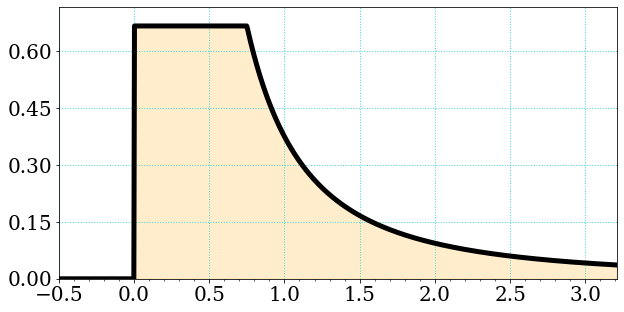
\includegraphics[width=0.9\textwidth]{2_53d11}
\end{figure}


3) вероятность равна:
$
\P(0,\!182\leqslant Z\leqslant 1,\!21)=
0,\!56852.
$


\item


(10) Известно, что доля возвратов по кредитам в банке имеет распределение $F(x) = x ^{\beta}, 0 \leqslant x \leqslant 1$.
Наблюдения показали, что в среднем она составляет $88,8889\%$. Методом моментов оцените параметр $\beta$ и
вероятность того, что она опуститься ниже $89\%$




Найдём плотность рапределения как интеграл от ФР, а дальше всё и вовсе простою Ответ: $3936588805702081$


\item

    
    Создайте эмперические совокупности  $\mathtt{\text{cos}}$ и $\mathtt{\text{log}}$ вида $\mathtt{\text{cos}}(1),\mathtt{\text{cos}}(2), ..., \mathtt{\text{cos}}(98) $ и $\mathtt{\text{log}}(1),\mathtt{\text{log}}(2), ..., \mathtt{\text{log}}(98). $

    Найдите эмпирическое среднее и эмпирическое стандартное отклонение совокупности $\mathtt{\text{cos}}$, её четвёртый эмпирический центральный момент и эмпирический эксцесс.

    Кроме того, найдите эмпирический коэффициент корреляции признаков $\mathtt{\text{cos}}$ и $\mathtt{\text{log}}$ на совокупности натуральных чисел от $1$ до $98$.
    


    
    Используя

	$E(X) = sum(X) / n$

	$Var(X) = E(X^2) - [E(X)]^2$

	$\mu_4(X) = E((X-E(X))^4)$

	$Ex = \frac{\mu_4(X)}{[\sigma(X)]^4} - 3$

	$r_{xy} = \frac{E(XY) - E(X) * E(Y)}{\sigma(X) * \sigma(Y)}$

    рассчитаем искомые значения.

    Ответы: $-0.01464, 0.70686, 0.37349, -1.50394, 1.0 \cdot 10^{-5}$.

    

\item


(10) Эмпирическое распределение признаков $X$ и $Y$ на генеральной совокупности $\Omega$ задано таблицей частот  
 
\begin{tabular}{ | c | c | c | c | }
\hline
 & $Y = 2$ & $Y = 4$ & $Y = 5$  \\ \hline
$X = 200$ & $17$ & $3$ & $13$\\ \hline
$X = 300$ & $21$ & $23$ & $23$\\
\hline
\end{tabular}

Из $\Omega$ случайным образом без возвращения извлекаются $10$ элементов. 
Пусть $\bar X$ и $\bar Y$ – средние значения признаков на выбранных элементах. 
Требуется найти: 1) математическое ожидание $\mathbb{E}(\bar Y)$; 2) стандартное отклонение $\sigma(\bar X)$ ; 
3) ковариацию $Cov(\bar X, \bar Y)$




1) математическое ожидание $\mathbb{E}(\bar Y)$: $3.6$ 
2) стандартное отклонение $\sigma(\bar X)$: $257.2355$
3) ковариацию $Cov(\bar X, \bar Y)$: $0.7091$


\item


(10) Пусть $X _{1}$, $X _{2}$, $X _{3}$, $X _{4}$ выборка из $N(\theta, \sigma ^{2})$. Рассмотрим две оценки параметра $\theta$:
\[\hat \theta _{1} = \frac{5X _{1} + 2X _{2} + X _{3} + 2X _{4}}{10}, \hat \theta _{1} = \frac{4X _{1} + 4X _{2} + X _{3} + X _{4}}{10}\]
a) Покажите, что обе оценки несмещенные.
б) Какая из оценок оптимальная?




Обе они несмещенные, потому что в числителе выходит в сумме 10.
Какая-то точно должна быть, а может и нет....


\end{enumerate}

\begin{figure}[H]
	Подготовил
	\hfill
	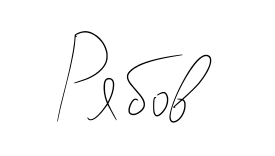
\includegraphics[width=2cm]{Prepared}
	П.Е. Рябов
\end{figure}


\begin{figure}[H]
	Утверждаю:\\
	Первый заместитель\\
	руководителя департамента\\
	Дата 01.06.2021
	\hfill
	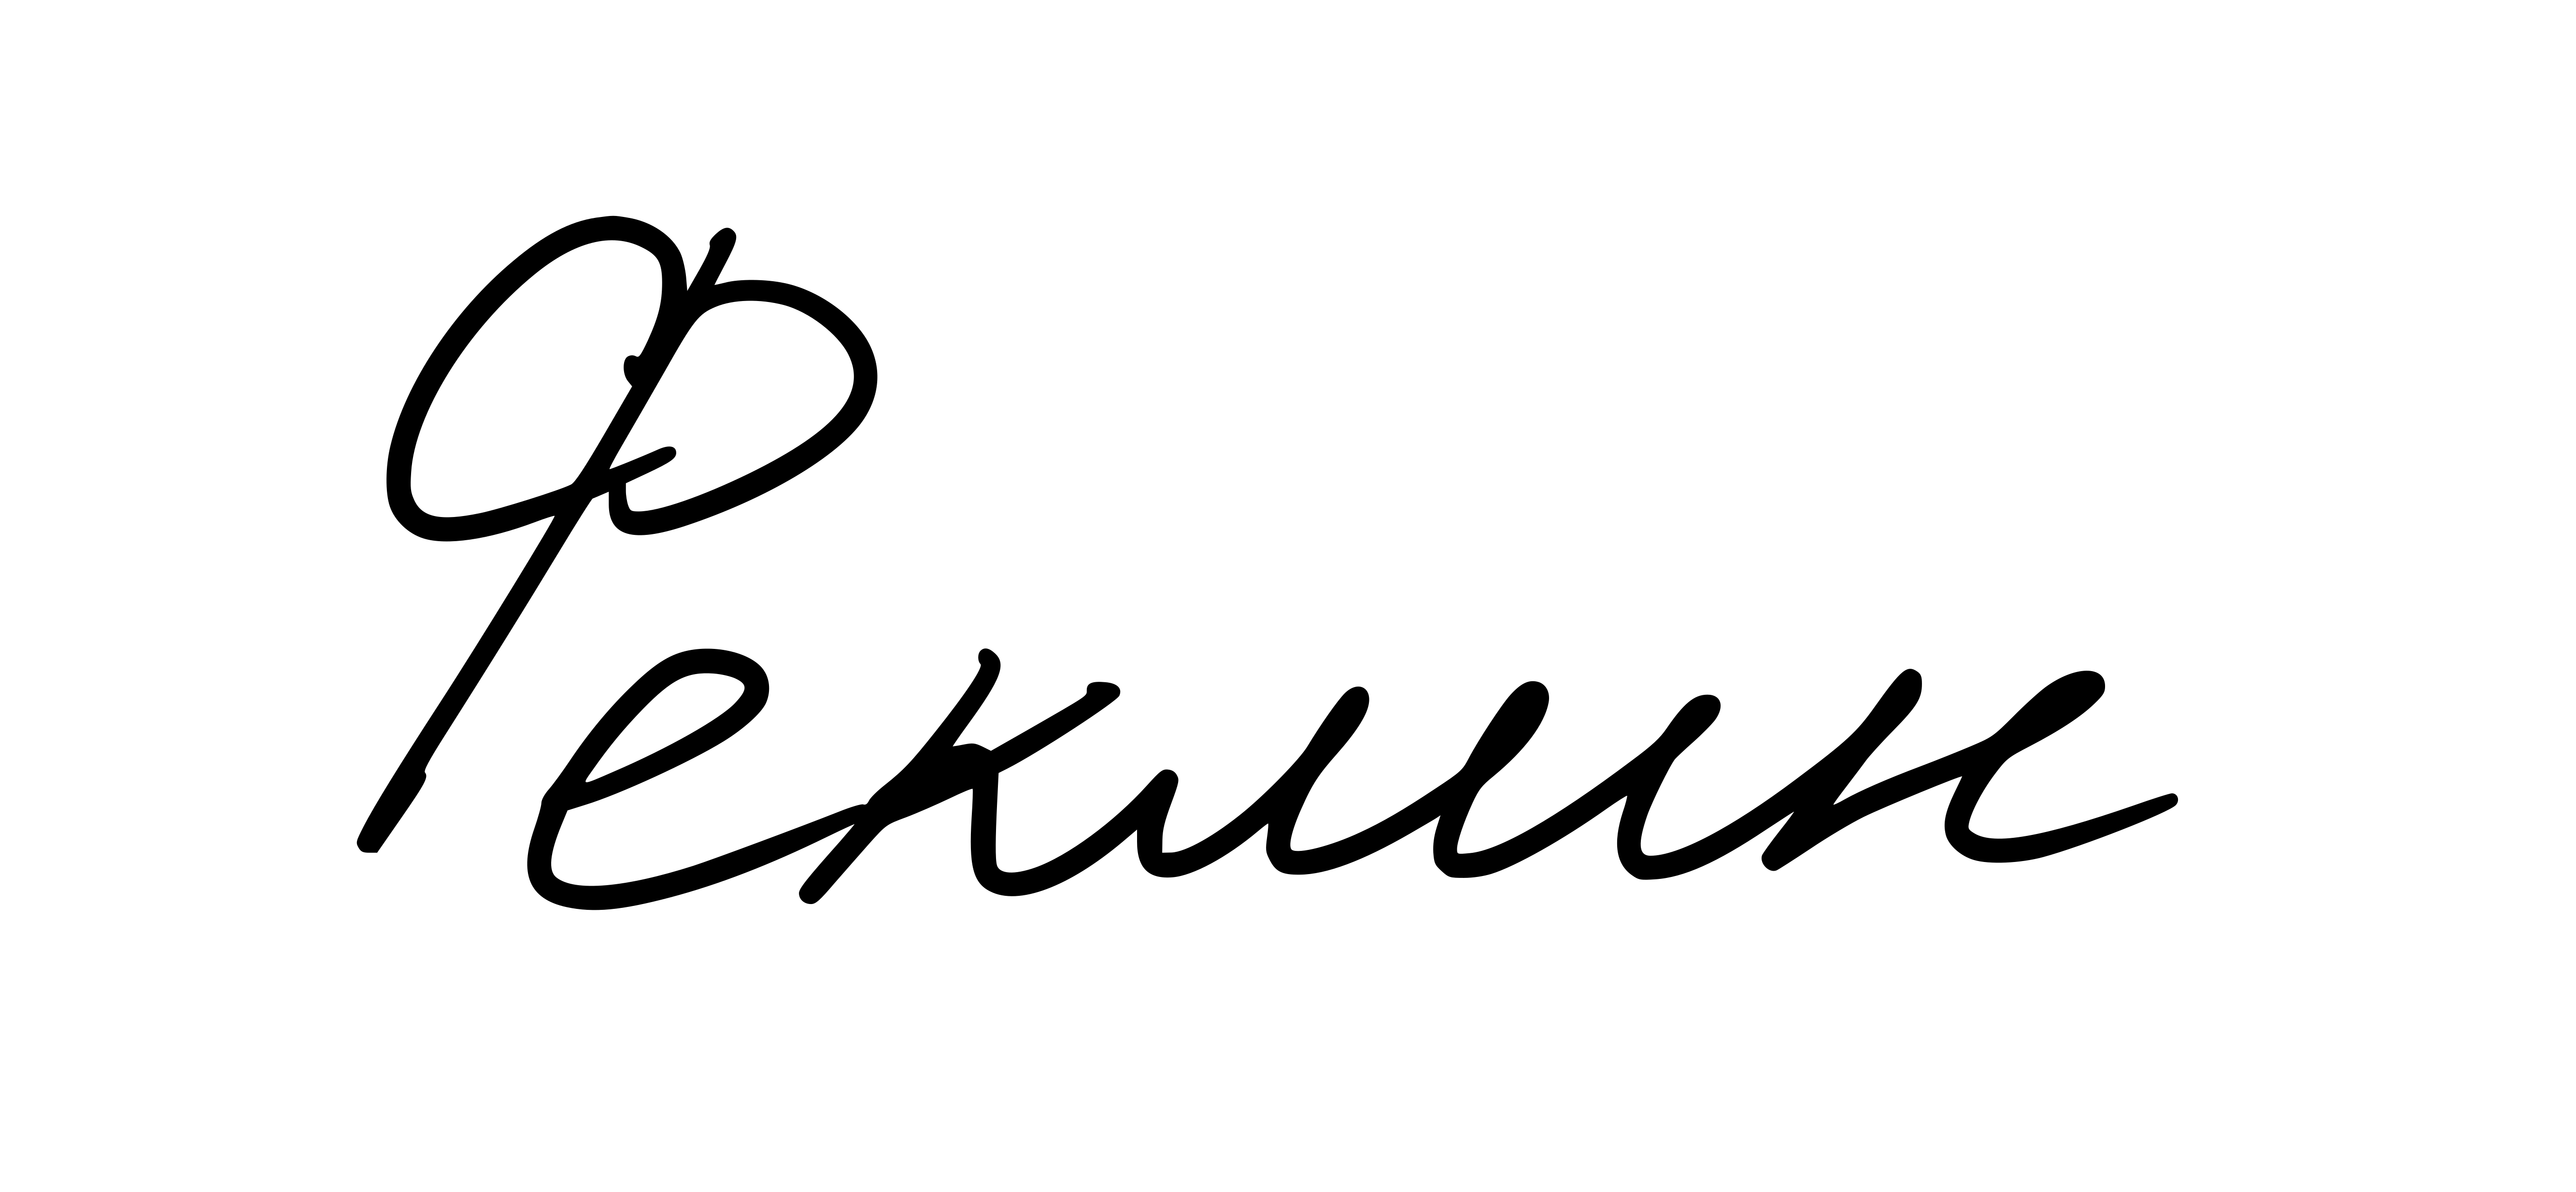
\includegraphics[width=2cm]{Approved}
	Феклин В.Г.
\end{figure}

\end{document}

